\documentclass[xcolor=dvipsnames]{beamer}
\usepackage{lmodern}
\usepackage[T1]{fontenc}
\usepackage[english]{babel}
\usepackage[utf8]{inputenc}

\usepackage{manfnt}
\usepackage{wasysym}
\usepackage{listings}
\usepackage{graphicx}
\usepackage{url}
\usepackage{ulem}
\usepackage{marvosym}
\usepackage{skull}
\usepackage{proof}
\usepackage{array}
\setbeamertemplate{navigation symbols}{}

\title[Landslide]{{\bf Systematic Testing: A New Perspective on Races}}
\subtitle[]{ {\em more clever than } ``\texttt{slaughter cho2}'' {\em since 2011.}}
\author[Ben Blum]{Ben Blum \texttt{(bblum@andrew.cmu.edu)}}

\institute[CMU 15-410]{Carnegie Mellon University - 15-410}
\date[]{2014, April 2}

\setbeamertemplate{footline}{\hspace*{.5cm}\scriptsize{\insertauthor\hspace*{50pt} \hfill\insertframenumber\hspace*{.5cm}}} 

\usecolortheme{seahorse}
\usecolortheme{rose}
\useoutertheme{infolines}

\usecolortheme[named=ForestGreen]{structure}

\newcommand\noob{\mathsf{noob}}
\newcommand\gibs{\mathsf{gibs}}
\newcommand\dps{\mathsf{dps}}
\newcommand\squig\rightsquigarrow
\newcommand\Coloneqq{\mathrel{\mathop{::}}=}
\newcommand\dmg{\text{\Laserbeam}}
\newcommand\delter\delta
\newcommand\alpher\alpha
\newcommand\defnor{\text{ }|\text{ }}

\newcommand\pimp{\mathop{\supset}}
\newcommand\pand{\mathop{\wedge}}
\newcommand\por{\mathop{\vee}}
\newcommand\ptrue{\top}
\newcommand\pfalse{\bot}

\newcommand\hilight[2]{\color{#1}#2\color{black}}
\definecolor{olivegreen}{RGB}{0,127,0}

\begin{document}
\normalem
\begin{frame}
	\titlepage
\end{frame}

%%%%%%%%%%%%%%%%%%%%%%%%%%%%%%%%%%%%%%%%%%%%%%%%%%%%%%%%%%%%%%%%%%%%%%%%%%%%%%%%
%%%%%%%%%%%%%%%%%%%%%%%%%%%%%%%%%%%%%%%%%%%%%%%%%%%%%%%%%%%%%%%%%%%%%%%%%%%%%%%%
%%%%%%%%%%%%%%%%%%%%%%%%%%%%%%%%%%%%%%%%%%%%%%%%%%%%%%%%%%%%%%%%%%%%%%%%%%%%%%%%

\newcommand\linegap{\vspace{0.2in}}
\newcommand\breakslide[1]{\begin{frame}{} \begin{center} #1 \end{center} \end{frame}}

\section{Introduction}
\subsection{Introduction}

\begin{frame}{Outline}
	\textbf{Theory: Seeing race conditions in a new way}
	\begin{itemize}
		\item Case study (example)
		\item The execution tree
		\item Preemption points
	\end{itemize}
	{\bf Technique: Systematic testing}
	% Say: A way of enumerating all possible interleavings of a concurrent test case.
	\begin{itemize}
		\item Requirements
		\item Challenges and feasibility
	\end{itemize}
	{\bf Tool: Landslide}
	\begin{itemize}
		\item How it works
		\item The user-tool relationship
		\item User study (that's you!)
			% !!! SAY !!! : If you are struggling, this is not for you, etc.
	\end{itemize}
\end{frame}

\subsection{Race Conditions}

% Say: Since I'm no longer a member of course staff, I'm allowed to give away a
% race condition that some of you might have, for the sake of example.

\begin{frame}[fragile]{Case Study}
	\begin{center}
	\begin{verbatim}
	    int thread_fork()
	    {
	        thread_t *child = construct_new_thread();
	        add_to_runqueue(child);
	        return child->tid;
	    }
	\end{verbatim}
	\end{center}

%	\begin{itemize}
%		\item On vanish, child's TCB is freed
%		\item Forking thread does use-after-free
%		\item Might return garbage instead of TID
%	\end{itemize}
\end{frame}

\begin{frame}{Thread Interleavings (``good'' case)}
	\begin{tabular}{|l|l|l}
		\cline{1-2}
		{\bf Thread 1} & {\bf Thread 2} & \\
		\cline{1-2}
		\texttt{spawn\_new\_thread} && \\
		\cline{1-2}
		\texttt{add\_to\_runqueue} && (new thread) \\
		\cline{1-2}
		\texttt{return child->tid} &&  \\
		\cline{1-2}
		& \texttt{vanish} & \\
		\cline{1-2}
		& (TCB gets freed) & (voluntary reschedule) \\
		\cline{1-2}
	\end{tabular}
\end{frame}

\begin{frame}{Thread Interleavings (race condition)}
	\begin{tabular}{|l|l|l}
		\cline{1-2}
		{\bf Thread 1} & {\bf Thread 2} & \\
		\cline{1-2}
		\texttt{spawn\_new\_thread} && \\
		\cline{1-2}
		\texttt{add\_to\_runqueue} && (new thread + preempted) \\
		\cline{1-2}
		& \texttt{vanish} & \\
		\cline{1-2}
		& (TCB gets freed) & (voluntary reschedule) \\
		\cline{1-2}
		\texttt{return child->tid} && (bad!) \\
		\cline{1-2}
	\end{tabular}
\end{frame}

\begin{frame}{Testing}
	How can programmers be confident in their code's correctness?
	\begin{itemize}
		\item Unit tests
		\begin{itemize}
			\item good for basic functionality, bad for concurrency
		\end{itemize}
		\item Stress tests
		\begin{itemize}
			\item state of the art in 15-410
		\end{itemize}
		\item Theorem proving
		\begin{itemize}
			\item heavy burden on the programmers
		\end{itemize}
		\item Releasing to paying customers and worrying about correctness later
	\end{itemize}
	\linegap

	{\bf Motivation}: Can we do better than stress testing?
\end{frame}

\begin{frame}{Testing Mechanisms}
	\textbf{Stress testing}: \texttt{slaughter cho2} and friends
	\begin{itemize}
		\item Attempting to exercise as many interleavings as practical
		\item Exposes race conditions at random
		\begin{itemize}
			\item ``If a preemption occurs at just the right time\ldots''
		\end{itemize}
		\item Cryptic panic messages or machine reboots
	\end{itemize}
	\linegap
	What if\ldots
	\begin{itemize}
		\item Make educated guesses about when to preempt
		\item Preempt enough times to run {\em every single} interleaving
		\item Tell the story of what {\em actually happened}.
		\item Overlook fewer bugs!
	\end{itemize}
	% Say: At the end of this lecture, I'm going to be looking for some among you...
\end{frame}

\breakslide{\Large A different way of looking at race conditions\ldots}

\begin{frame}{Execution Tree}
	\begin{center}
		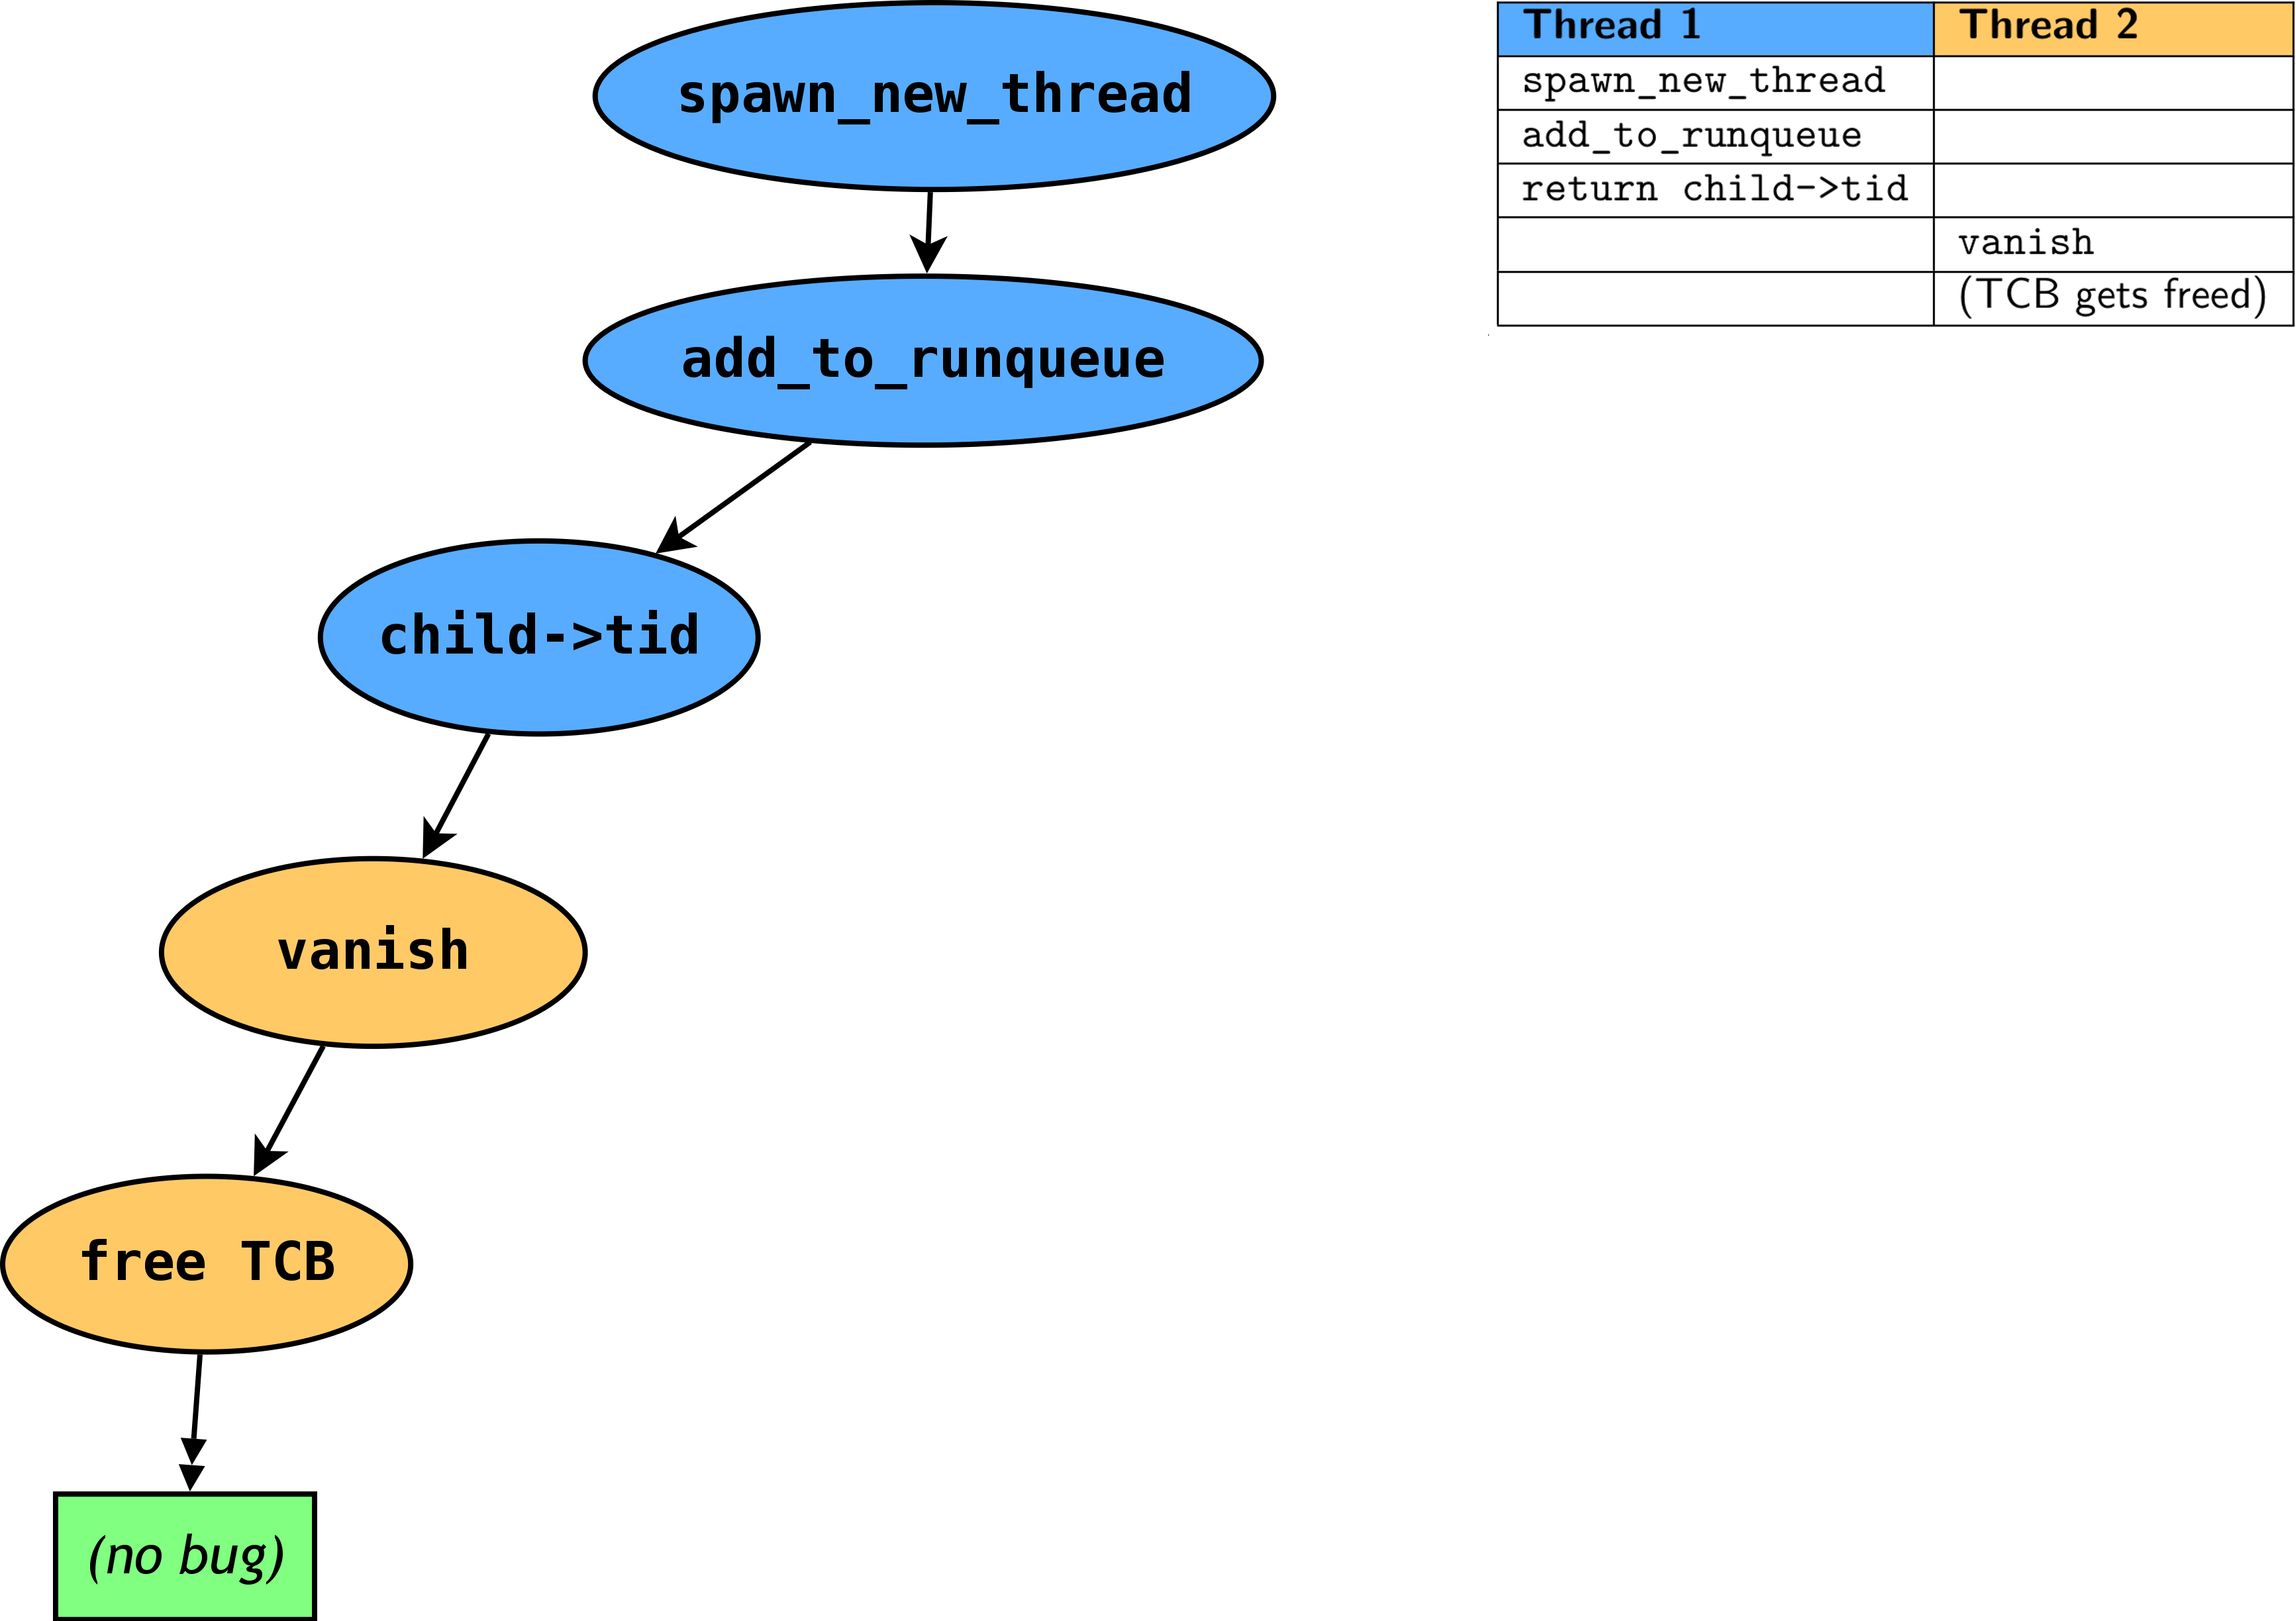
\includegraphics[width=0.9\textwidth]{threadfork0.png}
	\end{center}
\end{frame}
\begin{frame}{Execution Tree}
	\begin{center}
		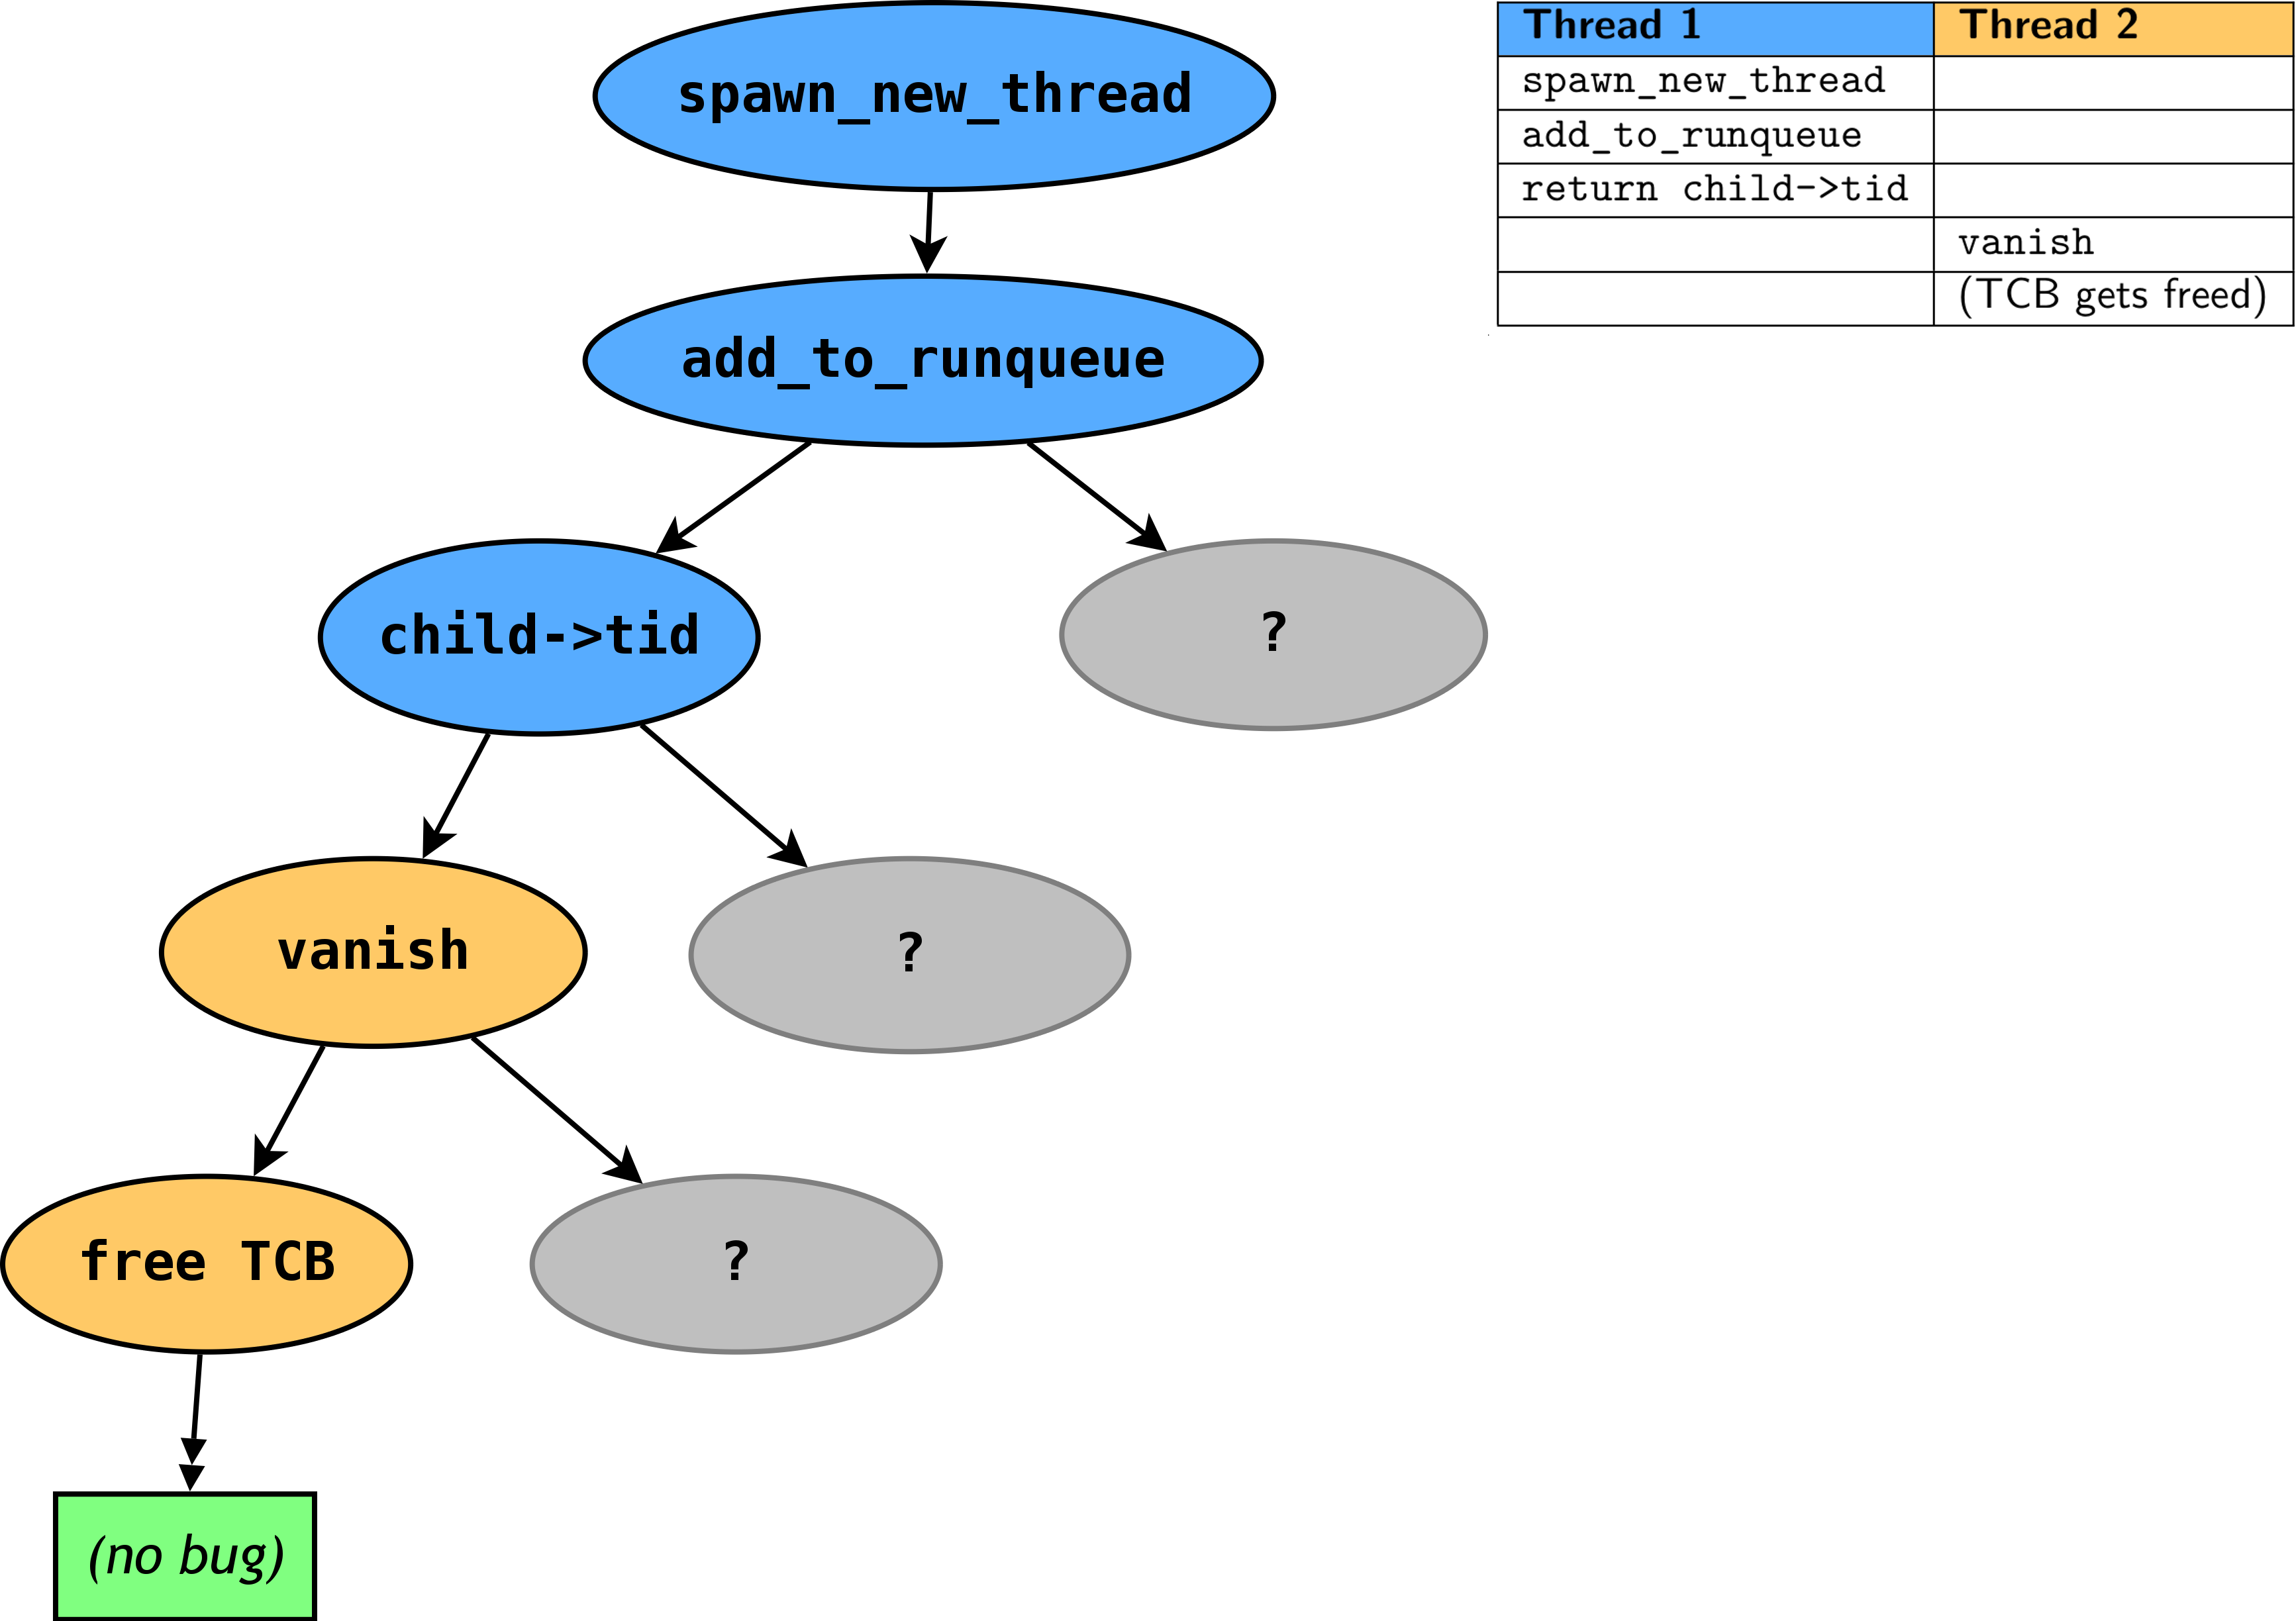
\includegraphics[width=0.9\textwidth]{threadfork05.png}
	\end{center}
\end{frame}
\begin{frame}{Execution Tree}
	\begin{center}
		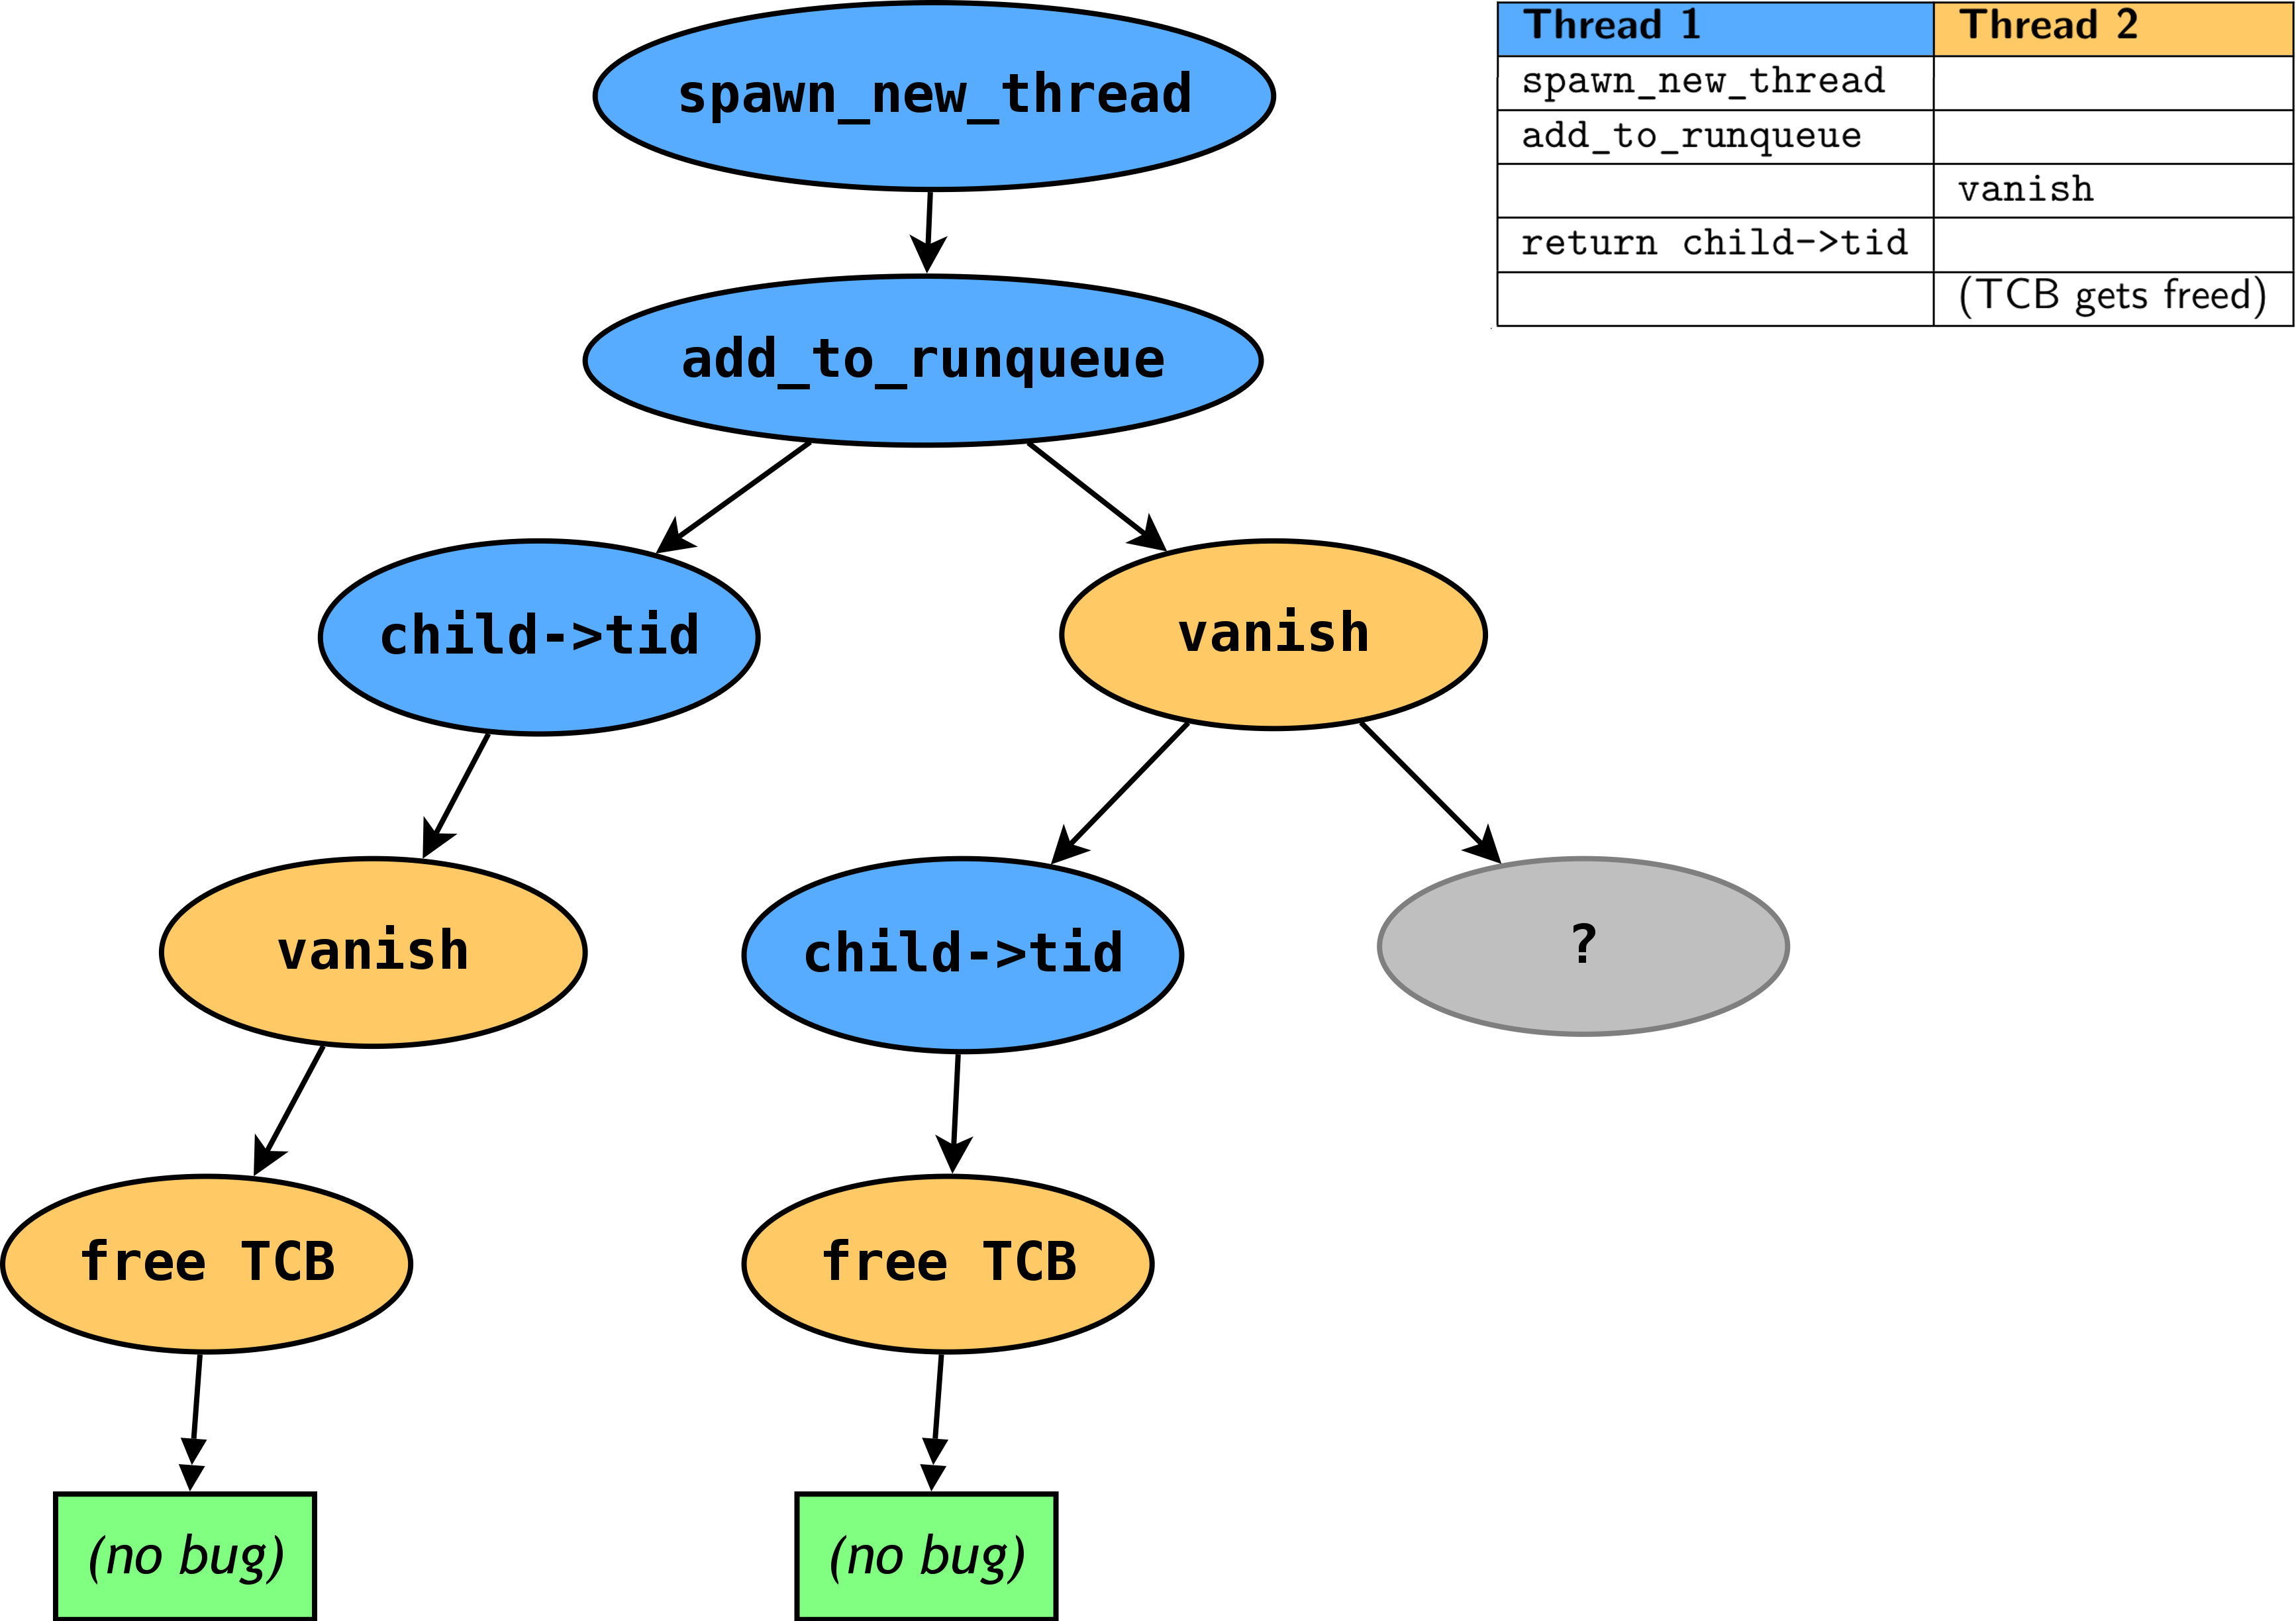
\includegraphics[width=0.9\textwidth]{threadfork1.png}
	\end{center}
\end{frame}
\begin{frame}{Execution Tree}
	\begin{center}
		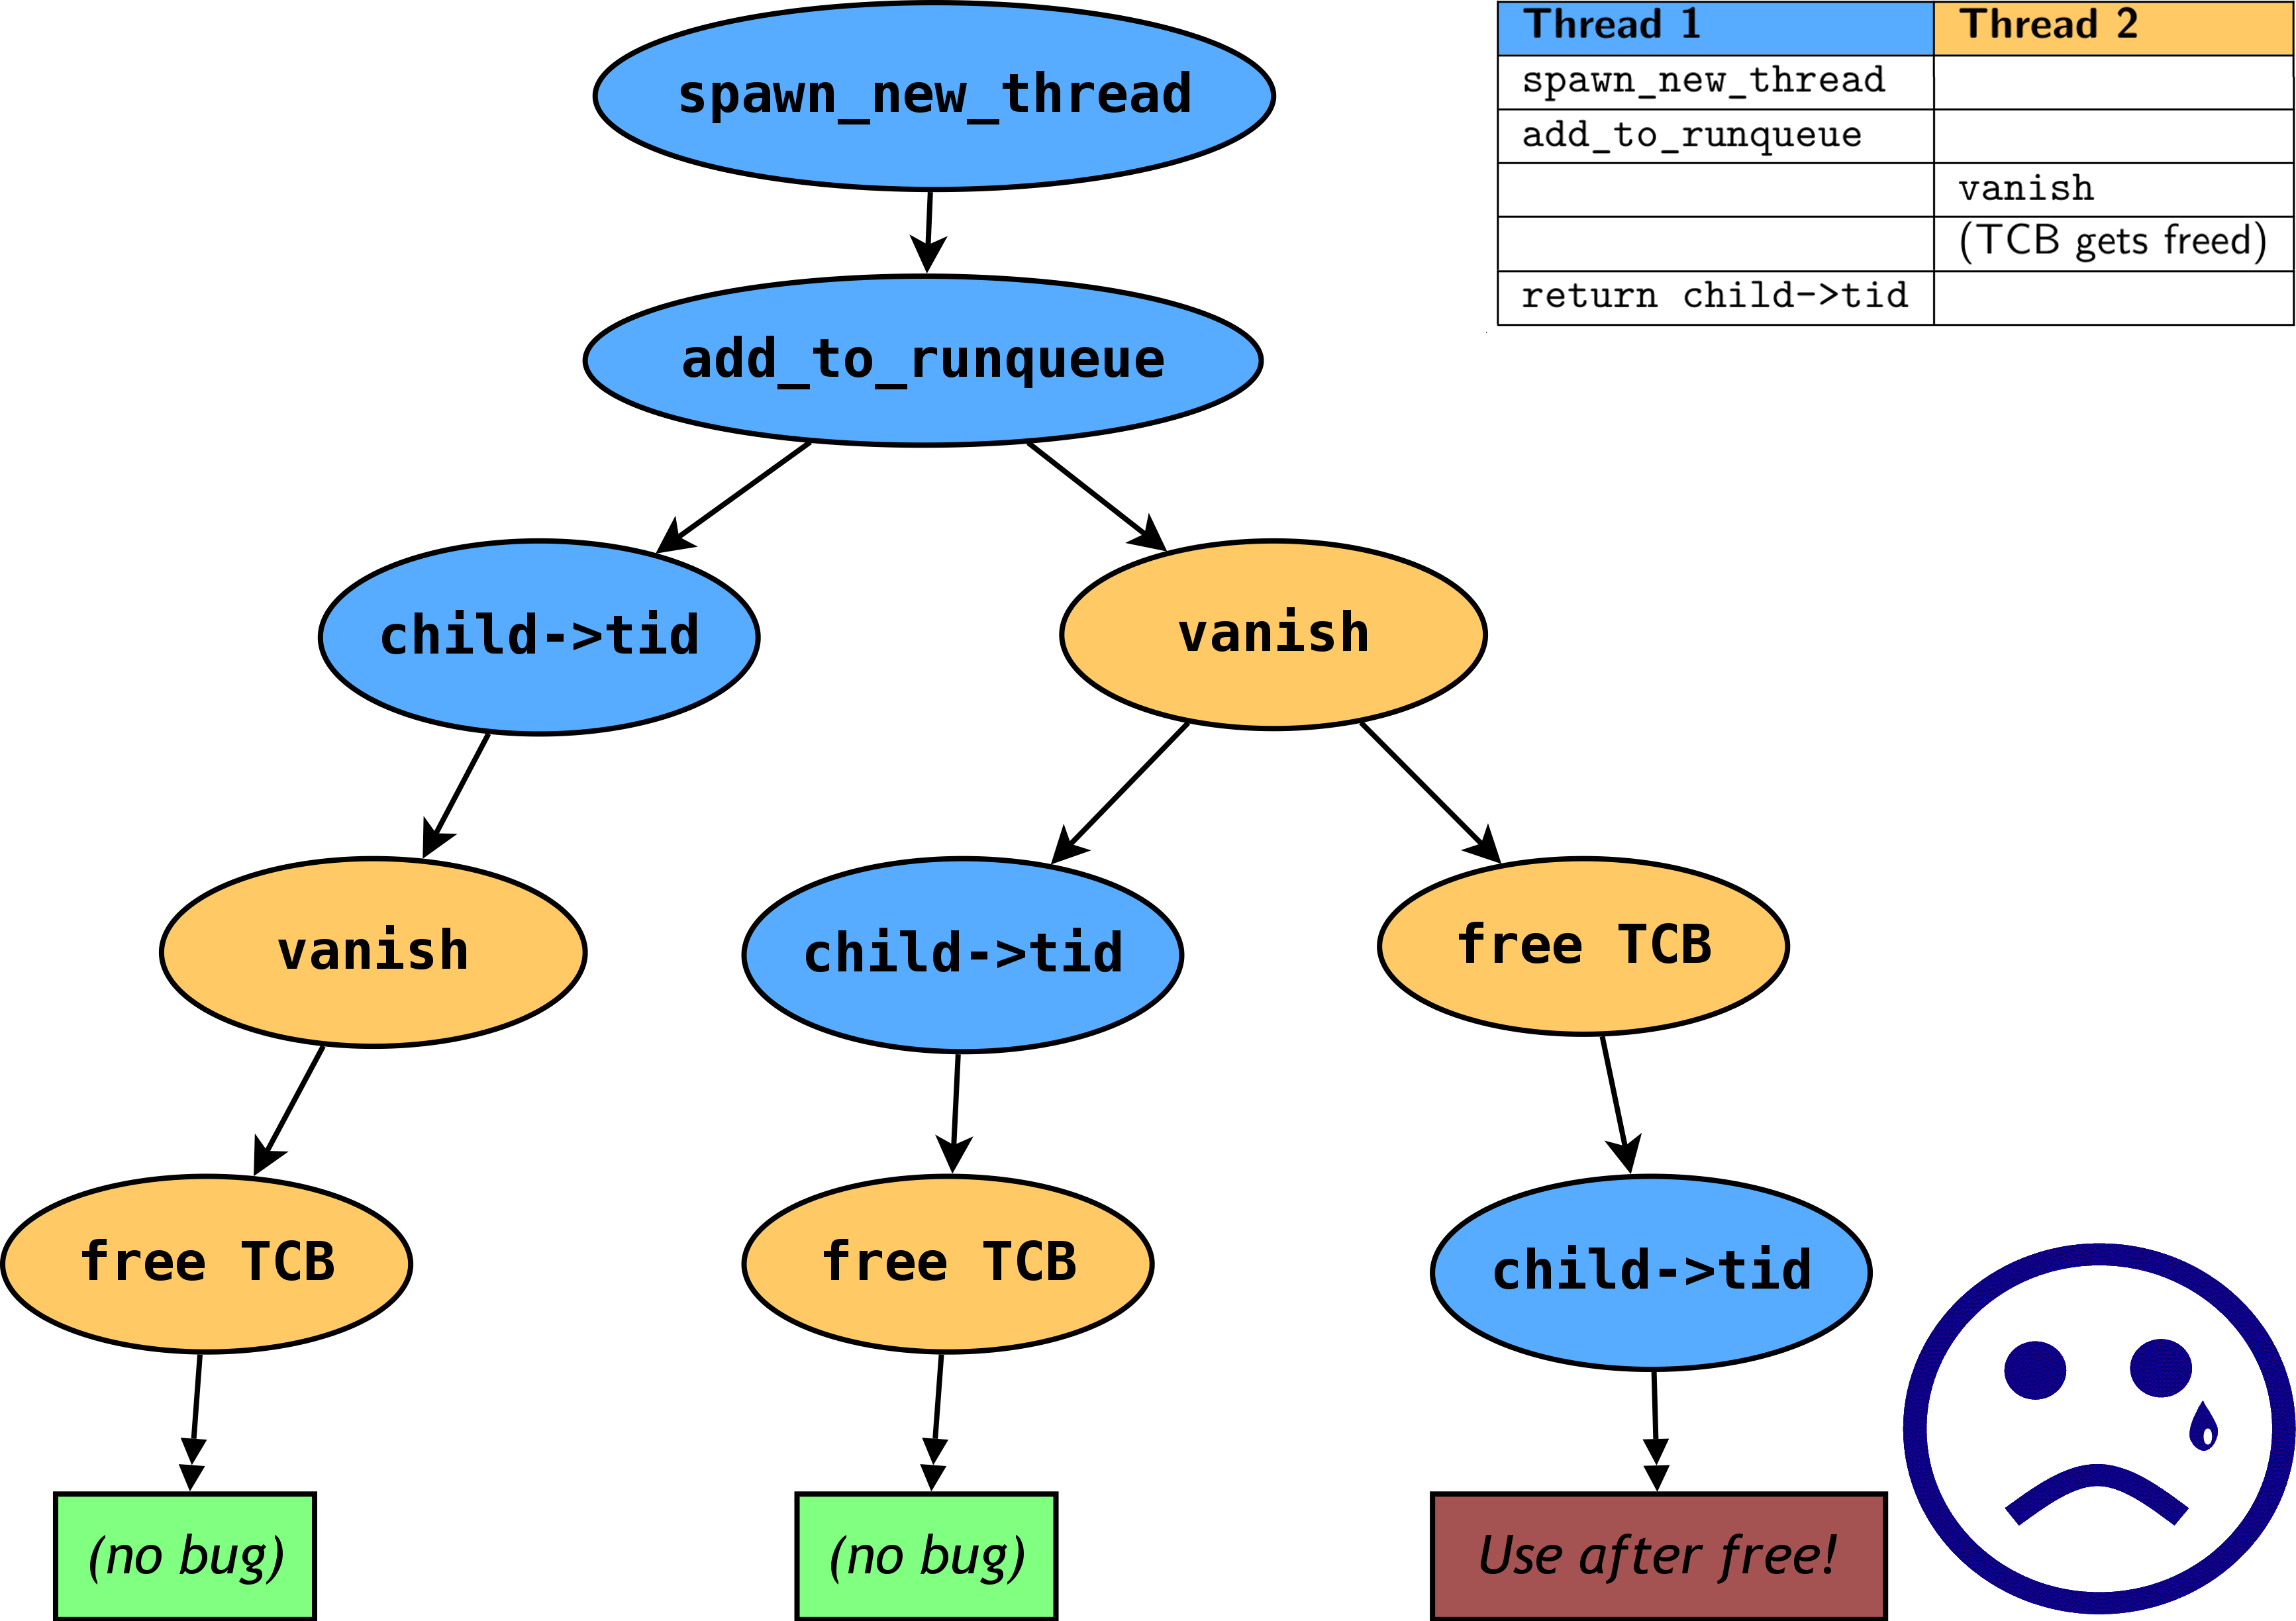
\includegraphics[width=0.9\textwidth]{threadfork2.png}
	\end{center}
\end{frame}

% Say: Obviously we want to be able to always run the third path. But knowing
% that ahead of time is impossible.
% Say: Okay, now what if we could build a tool that could ``systematically''
% explore this tree, and find the branch with the bug in it? What would such a
% tool need to be able to do?

%%%%%%%%%%%%%%%%%%%%%%%%%%%%%%%%%%%%%%%%%%%%%%%%%%%%%%%%%%%%%%%%%%%%%%%%%%%%%%%%
%%%%%%%%%%%%%%%%%%%%%%%%%%%%%%%%%%%%%%%%%%%%%%%%%%%%%%%%%%%%%%%%%%%%%%%%%%%%%%%%
%%%%%%%%%%%%%%%%%%%%%%%%%%%%%%%%%%%%%%%%%%%%%%%%%%%%%%%%%%%%%%%%%%%%%%%%%%%%%%%%

\section{Systematic Testing}

\breakslide{\Large Systematic Testing}

\begin{frame}{Systematic Testing - The Big Picture}
	\textbf{Goal: Force the system to execute every possible interleaving.}
	% Say: checking for crashes/memory errors/etc in each one.
	\begin{itemize}
		\item At end of each branch, rewind system and restart test.
		\item Artificially add preemptions to test different thread interleavings.
		\item Intuitively: Generate many ``tabular execution traces''.
	\end{itemize}
	\pause
	\linegap

	Okay, wait a sec...
	\begin{itemize}
		\item How can you possibly execute {\em every possible} interleaving?
		\item How can you know where preempting matters most?
	\end{itemize}
\end{frame}

\begin{frame}{Preemption Points}
	\textbf{Preemption points} (PPs) are code location where being preempted may cause different behaviour.
	\begin{itemize}
		\item IOW, somewhere that interesting interleavings can happen around.
	\end{itemize}
	\linegap

	Systematic tests are {\em parameterized} by the set of PPs.
	\begin{itemize}
		\item If there are $n$ PPs and $k$ threads, state space size is $n^k$.
		\item Need to choose the set of PPs very carefully for test to be effective.
	\end{itemize}
\end{frame}


\begin{frame}{Preemption Points}
	What does ``all possible interleavings'' actually mean?

	\linegap
	One extreme: Preempt at every instruction
	\begin{itemize}
		\item {\em Good news}: Will find every possible race condition.
		\item {\em Bad news}: Runtime of test will be impossibly large.
	\end{itemize}
	\linegap

	Other extreme: Nothing is a preemption point
	\begin{itemize}
		\item {\em Good news}: Test will finish quickly.
		\item {\em Bad news}: Only one execution was checked for bugginess.
		\begin{itemize}
			\item No alternative interleavings explored.
			\item Makes ``no race found'' a weak claim.
		\end{itemize}
	\end{itemize}
	\linegap

	Is there a ``sweet spot''?
\end{frame}

\begin{frame}{Preemption Points}
	Sweet spot: Insert a thread switch everywhere it ``might matter''.

	\linegap
	When do we fear being preempted?
	\begin{itemize}
		\item Threads becoming runnable (\texttt{fork()}, \texttt{cond\_signal()}, etc.)
			\begin{itemize}
				\item Preemptions may cause it to run before we're ready
			\end{itemize}
		\item Synchronization primitives (\texttt{mutex\_lock()}/\texttt{unlock()}, etc.)
			\begin{itemize}
				\item If used improperly\ldots
			\end{itemize}
		\item Unprotected shared memory accesses % Say: more on this later.
			\begin{itemize}
				\item May result in data structure corruption
			\end{itemize}
	\end{itemize}
	\linegap

	%%%% Not anymore! :D
	%Finding the sweet spot is a joint effort between programmer and tool. (More on this later.)
\end{frame}

\subsection{Challenges}

%% TODO -- left off working on slides here.

% TODO TODO 2014: move this slide below the "preemption point" series, to after "controlling scheduling decisions", so it can be a two-parter -- "What are the two parts necessary to navigate a path through the tree?"
\begin{frame}{Execution Tree Exploration}
	Important point: When does a branch end?
	\begin{itemize}
		\item All threads run to completion, or
		\item A bug is detected % Say: more on this later.
	\end{itemize}
	\linegap
	{\bf Backtracking}:
	\begin{itemize}
		\item Identify a preemption point to replay differently
		\item Reset machine state and start over
		\item Replay test from the beginning, with different preemptions
	\end{itemize}
\end{frame}

\begin{frame}{Controlling Scheduling Decisions}
	How do we control which thread runs when?
	\linegap

	In other words, what sources of nondeterminism must we control?

	\begin{itemize}
		\item Device interrupts/input
			\begin{itemize}
				\item Disk drivers: when disk reads finish
				\item Ethernet drivers: when packets arrive
			\end{itemize}
		\item To control thread switches in a 410 kernel, vary when clock ticks happen.
	\end{itemize}
\end{frame}

% TODO TODO 2014: this slide can be deleted
\begin{frame}{Memory Interposition}
	How do we detect race-induced heap corruption?
	\linegap

	In order to find use-after-free, need to know:
	\begin{itemize}
		\item When objects are \texttt{free()}d
		\item When threads access shared memory in the heap
	\end{itemize}
	\linegap

	Solution: Keep track of all memory events
	\begin{itemize}
		\item All calls to \texttt{malloc}/\texttt{free}
		\item All shared memory reads/writes
	\end{itemize}
\end{frame}

%%%%%%%%%%%%%%%%%%%%%%%%%%%%%%%%%%%%%%%%%%%%%%%%%%%%%%%%%%%%%%%%%%%%%%%%%%%%%%%%

\subsection{State Space Explosion}

\begin{frame}{State Space Explosion}
	Serious problem: State spaces grow exponentially
	\begin{itemize}
		\item With $p$ preemption points and $k$ runnable threads, size $p^k$.
		\item Threatens our ability to explore everything.
		\item Fortunately, some sequences result in identical states.
	\end{itemize}
	\linegap

	{\bf Partial Order Reduction} can help.
	\begin{itemize}
		\item Intuitively: After exploring each interleaving, identify ``equivalent'' alternatives and skip over them.
		\item Example follows\dots
	\end{itemize}
\end{frame}

\begin{frame}{State Space Explosion}
	\begin{center}
	\includegraphics[width=\textwidth]{undiamond0.png}
	\end{center}
\end{frame}
\begin{frame}{State Space Explosion}
	\begin{center}
	\includegraphics[width=\textwidth]{undiamond1.png}
	\end{center}
\end{frame}
\begin{frame}{State Space Explosion}
	\begin{center}
	\includegraphics[width=\textwidth]{diamond1.png}
	\end{center}
\end{frame}

%%%%%%%%%%%%%%%%%%%%%%%%%%%%%%%%%%%%%%%%%%%%%%%%%%%%%%%%%%%%%%%%%%%%%%%%%%%%%%%%
%%%%%%%%%%%%%%%%%%%%%%%%%%%%%%%%%%%%%%%%%%%%%%%%%%%%%%%%%%%%%%%%%%%%%%%%%%%%%%%%
%%%%%%%%%%%%%%%%%%%%%%%%%%%%%%%%%%%%%%%%%%%%%%%%%%%%%%%%%%%%%%%%%%%%%%%%%%%%%%%%

\section{Landslide}

\breakslide{\Huge Landslide}

\begin{frame}{About The Project}
	% 5th year MS since June 2011 % Say: planning to finish this may, hopefully
	My MS thesis project (2011-2012)
	\begin{itemize}
		\item {}[CMU-CS-12-118 -- \url{http://bblum.net/thesis.pdf}]
	\end{itemize}

	\linegap
	Now I'm a Ph.D. student\dots

	\linegap
	Working with Garth Gibson, Jiri Simsa

	\linegap
	{\bf Landslide}: Shows that your Pebbles are not as stable as you thought.
\end{frame}

%%%%%%%%%%%%%%%%%%%%%%%%%%%%%%%%%%%%%%%%%%%%%%%%%%%%%%%%%%%%%%%%%%%%%%%%%%%%%%%%

\subsection{How Landslide Works}

\begin{frame}{Landslide in Simics}
	As a Simics module, Landslide knows:
	\begin{itemize}
		\item Every instruction the kernel executes
		\item Every memory address the kernel reads/writes
	\end{itemize}
	\linegap
	Artificially causes timer interrupts to control scheduling

	\linegap
	Checkpointing/backtracking via Simics bookmarks (reverse execution)
\end{frame}

\begin{frame}{Anatomy}
	\begin{center}
	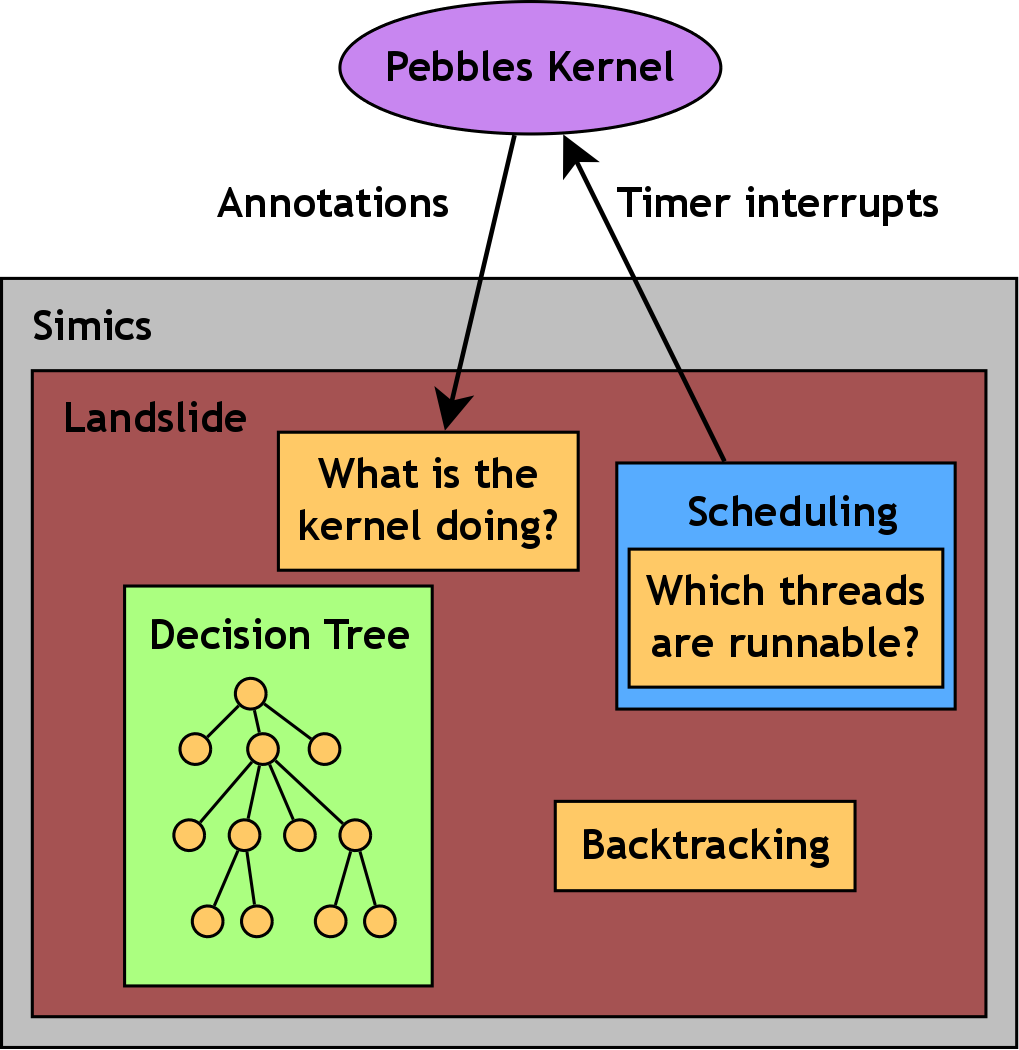
\includegraphics[width=0.6\textwidth]{landslide.png}
	\end{center}
\end{frame}

\begin{frame}{Identifying Bugs}
	Landslide can {\em definitely discover}:
	\begin{itemize}
		\item Kernel panics % Say: note: the better your asserts are..!
		\item Deadlock
		\item Use-after-free / double-free
	\end{itemize}
	\linegap
	Landslide can {\em reasonably suspect}:
	\begin{itemize}
		\item Memory leak
		\item Infinite loop (halting problem)
	\end{itemize}
\end{frame}

%%%%%%%%%%%%%%%%%%%%%%%%%%%%%%%%%%%%%%%%%%%%%%%%%%%%%%%%%%%%%%%%%%%%%%%%%%%%%%%%

\subsection{Using Landslide}

\breakslide{\Large Using Landslide}

\begin{frame}{Recruitment}
	% Say: So, this wasn't just a research talk
	This is something you can try!
	\linegap

	Mutual benefit
	\begin{itemize}
		\item Landslide may help you find bugs
		\item You help Ben evaluate his research
	\end{itemize}
\end{frame}

% TODO TODO 2014: move this slide later, to be neighbours with the other words of warning
\begin{frame}{Words of Warning}
	Finding race conditions is hard for humans.

	\linegap
	It is hard for computer programs too.

	\linegap
	Landslide is not an oracle.
\end{frame}

\begin{frame}{Annotating Your Kernel}
	Step 1
	\begin{center}
		{\small
		\begin{tabular}{l}
		\texttt{\hilight{olivegreen}{int}~thread\_fork() \{} \\
	        \texttt{~~~~\hilight{olivegreen}{thread\_t}~*child = construct\_new\_thread();} \\
		\texttt{~~~~\hilight{purple}{tell\_landslide\_forking}();~\hilight{blue}{/* A new thread was created.~*/}} \\
	        \texttt{~~~~add\_to\_runqueue(child);} \\
	        \texttt{~~~~return child->tid;} \\
		\texttt{\}} \\
		\texttt{\hilight{olivegreen}{void}~add\_to\_runqueue(\hilight{olivegreen}{thread\_t}~*t) \{} \\
		\texttt{~~~~\hilight{blue}{/* This thread is now runnable.~*/}} \\
		\texttt{~~~~\hilight{purple}{tell\_landslide\_thread\_on\_rq}(t->tid);} \\
		\texttt{~~~~...} \\
		\texttt{\}} \\
		\end{tabular}
		}
	\end{center}
	Your kernel needs to say when certain events happen, for example:
	\begin{itemize}
		\item When do threads become runnable / descheduled?
		\item When does the scheduler switch threads?
	\end{itemize}
\end{frame}

\begin{frame}{Configuring Landslide}
	Step 2
	\begin{center}
		{\small
		\begin{tabular}{l}
		\texttt{\hilight{blue}{\# What test case to run?}} \\
		\texttt{\hilight{black}{TEST\_CASE}=\hilight{olivegreen}{"double\_thread\_fork"}} \\
		\texttt{} \\
		\texttt{\hilight{blue}{\# The names of some important functions~~~~~~~~~~~}} \\
		\texttt{\hilight{black}{TIMER\_WRAPPER}=\hilight{olivegreen}{"timer\_handler\_wrapper"}} \\
		\texttt{\hilight{black}{CONTEXT\_SWITCH}=\hilight{olivegreen}{"ctx\_switch"}} \\
		\texttt{} \\
		\texttt{\hilight{blue}{\# What functions to pay attention to?}} \\
		\texttt{within\_function \hilight{olivegreen}{"thread\_fork"}} \\
		\texttt{within\_function \hilight{olivegreen}{"vanish"}} \\
		\end{tabular}
		}
	\end{center}
	\linegap

	Fill out \texttt{config.landslide} with design details and names of important functions

	% Fill in two implementation-dependent C functions in Landslide ($\le$10 lines)
	% Say: Which depend on your kernel's specific implementation
\end{frame}

\begin{frame}{Configuring Preemption Points}
	Landslide automatically identifies a minimal set of preemption points.
	\begin{itemize}
		\item It might find bugs.
		\item It might overlook more fine-grained interleavings.
	\end{itemize}
	\linegap
	With help from you, it could find more.
	\begin{itemize}
		\item Optional annotation: \texttt{tell\_landslide\_preempt()}
		\item Hints to where a context switch should be forced.
		\item Inside every call to \texttt{mutex\_lock}\ldots
	\end{itemize}
\end{frame}

% TODO TODO 2014: hopefully, update this with a tabular format in a semester's time!
\begin{frame}{And Hopefully\dots}
	\begin{center}
	{\small
        \begin{tabular}{l}
        \texttt{\hilight{red}{USE AFTER FREE - read from 0x199630 at eip 0x104264}} \\
        \texttt{Heap contents:~\{...\}} \\
        \texttt{[0x199630 | 4140] was allocated by TID3 at (...)} \\
        \texttt{~~~~~~~~~~~~~~~~~~~~~~and freed by TID4 at (...)} \\
        \texttt{\hilight{red}{****~~~~~~A bug was found!~~~~~****}} \\
        \texttt{\hilight{red}{**** Preemption trace follows.~****}} \\
        \texttt{\hilight{olivegreen}{1:~~TID 3 -{}-> TID 4}} \\
        \texttt{~~~~TID3 at 0x105a10 in \hilight{blue}{context\_switch},} \\
        \texttt{~~~~~~~~~~~~0x1041f4 in \hilight{blue}{thread\_fork},} \\
        \texttt{~~~~~~~~~~~~0x10362b in \hilight{blue}{thread\_fork\_wrapper}} \\
        \texttt{\hilight{olivegreen}{2:~~TID 4 -{}-> TID 3}} \\
        \texttt{~~~~TID4 at 0x105a10 in \hilight{blue}{context\_switch},} \\
        \texttt{~~~~~~~~~~~~0x104681 in \hilight{blue}{yield},} \\
        \texttt{~~~~~~~~~~~~0x104570 in \hilight{blue}{vanish},} \\
        \texttt{~~~~~~~~~~~~0x103708 in \hilight{blue}{vanish\_wrapper}} \\
        \texttt{\hilight{red}{Current stack:}}\\
        \texttt{~~~~TID3 at 0x104209 in \hilight{blue}{thread\_fork},} \\
        \texttt{~~~~~~~~~~~~0x10362b in \hilight{blue}{thread\_fork\_wrapper}}
        \end{tabular}
	}

	\end{center}
\end{frame}

\breakslide{\Large Quick Demo}

% TODO more of these with screenshots

%\begin{frame}{Preemption Points (noticing a theme here?)}
%	Landslide is {\bf false negative}-oriented.
%	\begin{itemize}
%		\item If Landslide reports a bug, there is a bug for sure.
%			% Say: Well, except progress sense might be wrong.
%		\item If not,
%			\begin{itemize}
%				\item Maybe there was no race, or
%				\item Maybe your preemption points were not granular enough.
%			\end{itemize}
%	\end{itemize}
%\end{frame}
%\begin{frame}{Preemption Points (noticing a theme here?)}
%	Sometimes the default set will work.
%
%	Sometimes you need to tweak\ldots
%	\begin{itemize}
%		\item Ignore certain global mutexes
%		\item Whitelist or blacklist entire syscalls
%		\item (get creative)
%	\end{itemize}
%	Intuitively: focusing Landslide on relevant parts of the kernel.
%\end{frame}

%%%%%%%%%%%%%%%%%%%%%%%%%%%%%%%%%%%%%%%%%%%%%%%%%%%%%%%%%%%%%%%%%%%%%%%%%%%%%%%%

\subsection{User Study}

\begin{frame}{Last Year's Results}
	\begin{itemize}
		\item Worked with 5 groups
		\begin{itemize}
			\item \dots{}of which 4 put in enough time to make Landslide work
		\end{itemize}
		\linegap
		\item {\bf Investment}: about 2 to 3 hours
		\begin{itemize}
			\item Average 112 minutes doing required instrumentation
			\item Average 35 minutes configuring extra preemption points \& interpreting ``found a bug'' output
		\end{itemize}
		\pause
		\linegap
		\item {\bf Return}: All 4 groups found bugs in their kernels.
		\begin{itemize}
			\item All groups found deterministic bugs (e.g., use-after-free)
			\item 2 groups found race conditions (i.e., Landslide needed to backtrack)
		\end{itemize}
	\end{itemize}
\end{frame}

\begin{frame}{Words of Warning Again}
	\textbf{If you are already struggling, this will not ``save'' you.}
	\begin{itemize}
		\item False-negatives: not guaranteed to find races at all
		\item Research-quality: possibly difficult to integrate with your kernel
		\item Finishing the kernel project is more important.
	\end{itemize}
	\pause
	\linegap
	This is for you if:
	\begin{itemize}
		%\item Be expecting an A or a B
		\item You have already submitted
		\item You are using late days, but willing to work over Carnival
		%\item Be able to turn in without late days (if you really had to)
		\item You are taking p3extra, but you already pass the hurdle
		\item You are looking for\ldots
			\begin{itemize}
				\item That ``one pesky race''
				\item A race that stress-testing missed
				\item Or just familiarity with a new technique
			\end{itemize}
	\end{itemize}
\end{frame}

\begin{frame}{Recruitment - Kernel Requirements}
	Your kernel
	\begin{itemize}
		\item Must load the shell and run programs
		\item \texttt{fork},
			\texttt{exec},
			\texttt{vanish},
			\texttt{wait},
			\texttt{readline}
		\item Must pass the hurdle architectural requirements
		\begin{itemize}
			\item especially: must never spin-wait!
		\end{itemize}
		\item Should \texttt{assert()} important invariants
		\begin{itemize}
			\item Think of \texttt{panic()} as \texttt{tell\_landslide\_bug()}
		\end{itemize}
	\end{itemize}
\end{frame}

\begin{frame}{Recruitment}
	User study this week, by appointment (\texttt{bblum@cs.cmu.edu})

	\linegap
	Expect to spend:
	\begin{itemize}
		\item Up to 3 hours, just to try it out.
		\item 4-6 hours, if you find a bug and track it down.
		\item More, for multiple bugs or the truly dedicated\ldots
	\end{itemize}
	\linegap

	Give feedback (intuitive? frustrating? found bugs?)

	\linegap
	{\bf Watch \texttt{410.announce} for details!}
\end{frame}

\subsection{End}
\breakslide{\Large Questions?}

%%%%%%%%%%%%%%%%%%%%%%%%%%%%%%%%%%%%%%%%%%%%%%%%%%%%%%%%%%%%%%%%%%%%%%%%%%%%%%%%
%%%%%%%%%%%%%%%%%%%%%%%%%%%%%%%%%%%%%%%%%%%%%%%%%%%%%%%%%%%%%%%%%%%%%%%%%%%%%%%%
%%%%%%%%%%%%%%%%%%%%%%%%%%%%%%%%%%%%%%%%%%%%%%%%%%%%%%%%%%%%%%%%%%%%%%%%%%%%%%%%


% \section{Conclusion}
% \subsection{Conclusion}
% 
% \begin{frame}{Summary}
% 	\begin{itemize}
% 		\item
% 	\end{itemize}
% \end{frame}

\end{document}
%\begin{frame}{Partial Order Reduction}
%	\begin{center}
%	The next 6 slides won't be on the exam.
%
%		\Huge \dbend
%	\end{center}
%\end{frame}
%
%\begin{frame}{Partial Order Reduction}
%	A {\bf transition} is\ldots
%	\begin{itemize}
%		\item The sequence of instructions executed between choice points.
%	\end{itemize}
%	To express concurrency between transitions:
%	% Say: As a prerequisite for this algorithm, we need to build two sets to express the concurrency relations between the transitions
%	\begin{itemize}
%		\item Independence relation
%		\item Happens-before relation
%	\end{itemize}
%	% Say: This is hard, and I don't expect you to understand it during this lecture; you won't be tested on it or anything. My goal in presenting it is to convey how intensely cool the algorithm is, and hopefully you will keep thinking about it later. I'd be happy to answer questions about it later.
%\end{frame}
%
%\begin{frame}[fragile]{Partial Order Reduction - Independence Relation}
%	\begin{columns}[l]
%		\column{0.5\textwidth}
%		\begin{center}
%		\begin{verbatim}
%		void thread_A() {
%		    foo = 42;
%		}
%		void thread_B() {
%		    if (bar == 1337)
%		        print "Hello"
%		}
%		\end{verbatim}
%		\end{center}
%		\linegap
%
%		$A$ and $B$ are {\bf independent}.
%		\column{0.5\textwidth}
%		\begin{center}
%		\begin{verbatim}
%		void thread_A() {
%		    foo = 42;
%		}
%		void thread_C() {
%		    if (foo == 1337)
%		        print "Hello"
%		}
%		\end{verbatim}
%		\end{center}
%		\linegap
%
%		$A$ and $C$ {\bf conflict}.
%	\end{columns}
%\end{frame}
%
%\begin{frame}{Partial Order Reduction - Independence Relation}
%	Consider a trace of all shared memory reads/writes
%
%	\linegap
%	Two transitions (instruction sequences) $A$ and $B$ are independent iff:
%	\begin{itemize}
%		\item $Writes(A) \cap Writes(B) = \emptyset$
%		\item $Writes(A) \cap Reads(B) = \emptyset$
%		\item $Reads(A) \cap Writes(B) = \emptyset$
%	\end{itemize}
%\end{frame}
%
%\begin{frame}{Partial Order Reduction - Happens-before Relation}
%	\begin{columns}[l]
%		\column{0.5\textwidth}
%		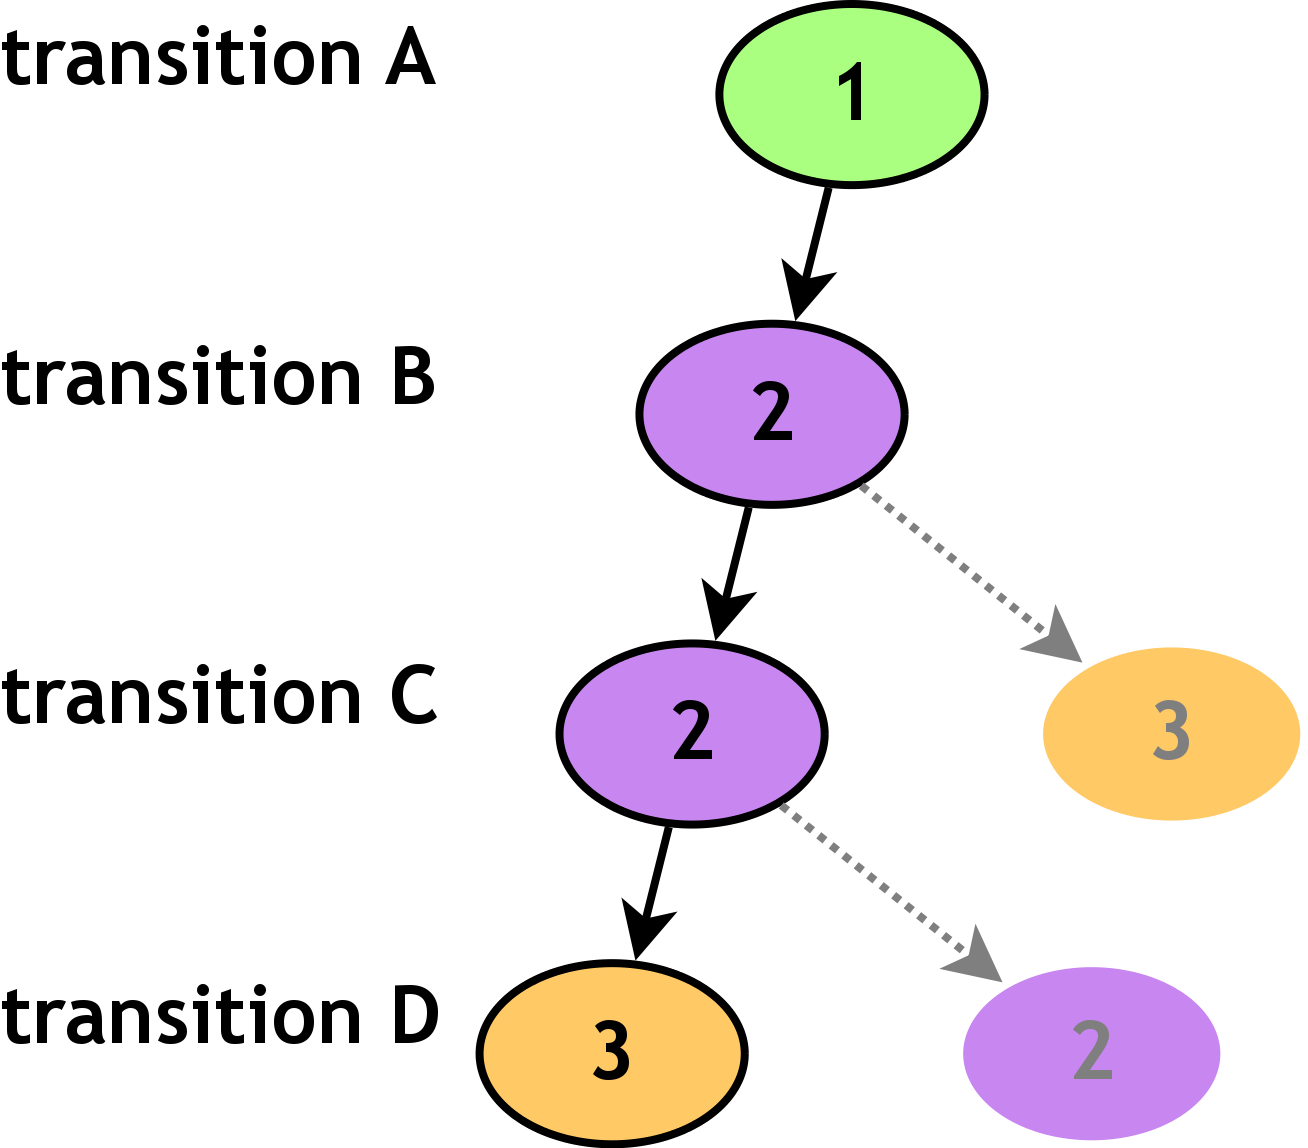
\includegraphics[width=\textwidth]{hb.png}
%		\column{0.5\textwidth}
%		Is a transition ``enabled'' by a previous one?
%		\begin{itemize}
%			\item $A$ enables $B$
%			\item $B$ enables $C$ (same thread)
%			\item $B$ enables $D$
%		\end{itemize}
%%		Transitive closure
%%		\begin{itemize}
%%			\item $HB^* = \{AB, AC, AD, BC, BD\}$
%%		\end{itemize}
%		$C$ and $D$ are {\bf concurrent}!
%	\end{columns}
%\end{frame}
%
%\begin{frame}{Partial Order Reduction - Tagging}
%	Run POR at the end of each branch
%	\begin{itemize}
%		\item Identify which branches to explore next
%		\item Tag only a subset of all branches (hopefully)
%	\end{itemize}
%\end{frame}
%
%\begin{frame}{Partial Order Reduction - Tagging}
%	For each transition $T$, find an {\bf evil ancestor} $E$:
%	\begin{itemize}
%		\item $E$ and $T$ are concurrent.
%		\item $E$ and $T$ are not independent.
%		\item Intuitively: $T$ and $E$ could be reordered, and might behave differently.
%	\end{itemize}
%	Find a {\bf good sibling} $G$ of $E$:
%	\begin{itemize}
%		\item $G$ is the same thread as $T$
%		% Say: (if no such sibling, all siblings)
%		\item Intuitively: Find a branch in which $T$ runs before $E$.
%	\end{itemize}
%	Explore tagged branches depth-first.
%\end{frame}
%
%\begin{frame}{Partial Order Reduction}
%	\begin{center}
%		{\Huge \dbend}
%		\linegap
%		\linegap
%		\linegap
%
%		Feel free to ask me about this later.
%	\end{center}
%\end{frame}

% TODO: run through an example

%%%%%%%%%%%%%%%%%%%%%%%%%%%%%%%%%%%%%%%%%%%%%%%%%%%%%%%%%%%%%%%%%%%%%%%%%%%%%%%%

%\subsection{Other Dynamic Techniques}
%
%\begin{frame}{Heuristic-Based Searching}
%	% Say: Note that this is beyond the scope of my personal project.
%	Maybe the tree is too big to search anyway?
%
%	\linegap
%	Search {\em most likely} branches first.
%	\begin{itemize}
%		\item ``Iterative Context Bounding''
%		\footnote{Microsoft Research - CHESS - Musuvathi et al.}
%		\begin{itemize}
%			\item Insight: Races tend to show up with few forced context switches.
%			\item Search branches with fewer preemptions first.
%		\end{itemize}
%		\item Find behaviours that are typical of buggy software.
%		\footnote{Stanford University - Dawson Engler}
%		\begin{itemize}
%			\item Different behaviour in different branches.
%				% Say: different all the time: no. different rarely: yes.
%			\item Use suspicious memory accesses as future choice points.
%		\end{itemize}
%	\end{itemize}
%	\linegap
%	Open research field, possibly my future work.
%\end{frame}
%
%% Say: I'm going to take a break from talking about systematic exploration to talk about other types of dynamic race detection - FIXME: if these slides fit in 60min.
%\begin{frame}{Data Race Detection}
%	Requires happens-before set and ``lock set''
%	\linegap
%
%	Two memory accesses $m_1$ and $m_2$ are a data race iff:
%	\begin{itemize}
%		\item Read/write or write/write to the same address, and
%		\item $(m_1,m_2) \not\in HB$, and
%		\item $Lock(m_1) \cap Lock(m_2) = \emptyset$
%	\end{itemize}
%\end{frame}
%\begin{frame}{Data Race Detection}
%	Data race detection vs systematic exploration
%	\begin{itemize}
%		\item More false positives
%			\begin{itemize}
%				\item (but still good style-checking!)
%			\end{itemize}
%		\item No false negatives
%		\item Still unable to find some types of bugs
%	\end{itemize}
%	\linegap
%	Hybrid approach? (future research)
%\end{frame}


